---------------------------------------------------

% What has been published on assembly.
Automated vessel platform assembly has been explored in various reasearches
\cite{mateos2019autonomous} % roboat latching / solution proposal
\cite{o2014self} % first usa large structures paper
\cite{paulos2015automated} % second usa large structures paper
, to allow formation without the need of a large team of vessel operators. 

% Introduce configuration adaptive control system: 
Assembled vessels together form a platform, which can, depending on the stiffness of connections, be considered a single body. Collaboration between vessels at platform level can improve dynamic response of the connected structure. Controlling a vessel platform that can have a different size and shape in an effective manner is a challenge which has been discussed in \cite{park2019coordinated} \cite{kayacan2019learning}. As two or more vessels connect into a platform, accurate modeling, controlling and coordinating become more complex. If the amount of configurations gets significantly high, gathering model parameters for every configuration becomes impossible, while also platform control effort needs to be allocated onto a large set of actuators. 

Consider the two systems earlier described, which can further be adressed as A and B and are illustrated in figure \ref{exaA} and \ref{exaB} respectively:
\begin{itemize}
	\item System A) An automated modular multi vessel system that performs self assembly.
	\item System B) An assembled vessel platform where it's actuators are controlled by using information of the configuration.
\end{itemize}

Benefits of both systems are desirable within one framework, as combining these systems into one allows engineers to utilize benefits from both. 

\begin{figure}[h!]
	\centering
	\makebox[\textwidth][c]{
		\begin{minipage}{0.45\textwidth}
			\centering
			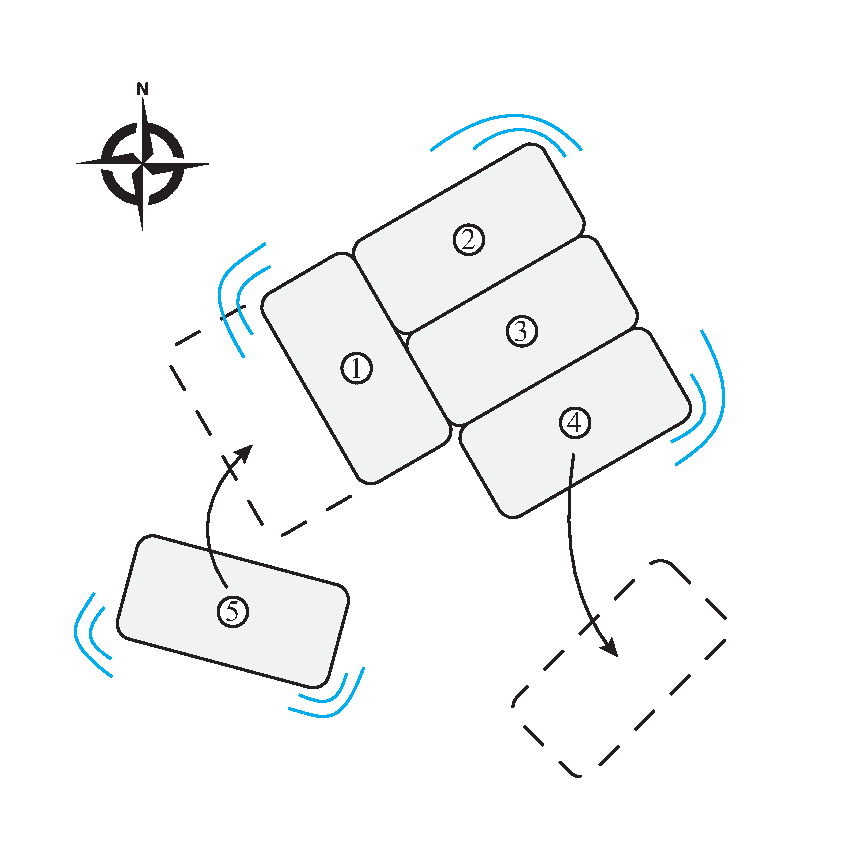
\includegraphics[width=0.95\textwidth]{img/intro_reconfiguration_square}
			\caption{Behavior A: Automatic reconfiguration of a vessel platform. Vessel 1,2,3 \& 4 are connected such that they form a platform. Arrows indicate movement of vessel 5 to connect, and disconnecting of vessel 4.}
			\label{exaA}
		\end{minipage}\hfill
		\begin{minipage}{0.45\textwidth}
			\centering
			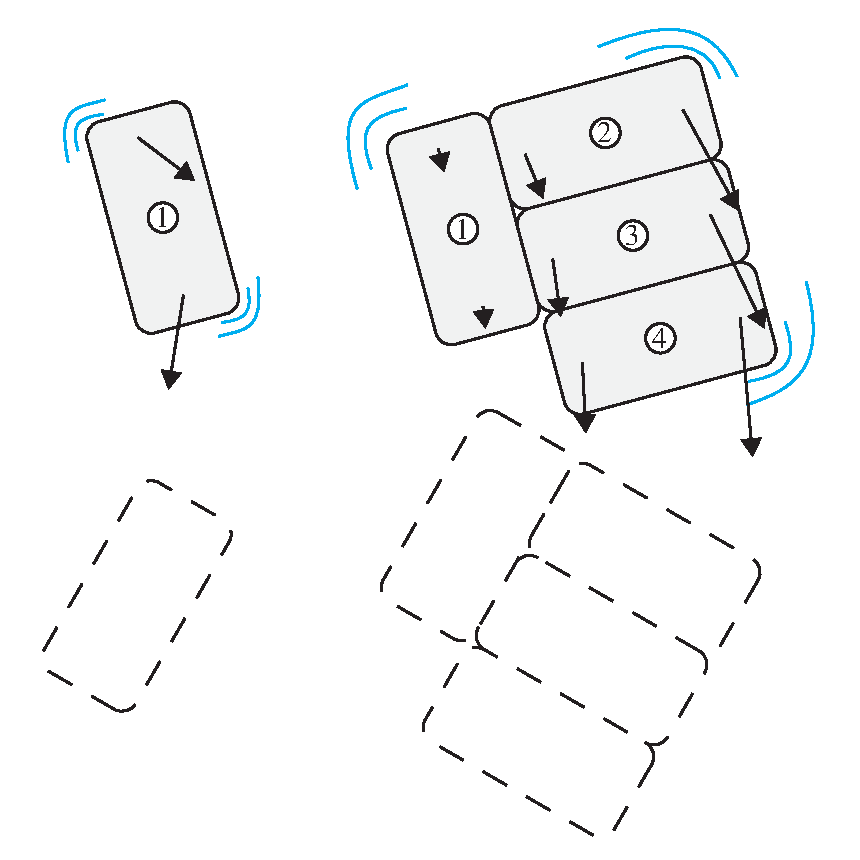
\includegraphics[width=0.95\textwidth]{img/intro_adaptation_square}
			\caption{Behavior B: Fleet control that adapts on platform configuration. The left vessel is configured in the simplest way, and operates alone. Four vessels on the right collaborate to move the connected vessel platform. Arrows illustrate forces generated by thrusters. }
			\label{exaB}
		\end{minipage}
	}
\end{figure}

\section{Problem statement}
It would be useful for developers to know what system requirements, characteristics and constraints emerge from implementing a framework with behavior of system A and B. This information can be used to make well informed, effective, scalable, interoperable and long term beneficial design choices. 

Literature on both systems is available, but there is a lack of content that describes the effect of combining both systems into one, which is the gap of knowledge that this thesis will adress. The research objective of this work is to develop, implement and evaluate a fleet control system performing self assembly and configuration adaptive control within a single framework. 
%The goal of this work is to create a benchmark for automated self-assembling vessel frameworks able to perform platform configuration dependent collaboration.
\newpage
\section{Approach}
To move torwards realizing implementation of automated vessel platforming systems, this paper strives to fill the gap of knowledge on implementation of automated assembling vessel platforms with configuration adaptive control strategies by seeking to answer the following questions:\\

\noindent {\large\textbf{ Main research question}}
\begin{itemize}
	\item How can a fleet of modular surface platform vessels be controlled to achieve automated assembly and configuration-dependent platform control?
\end{itemize}

%is split into several subquestions, starting with two regarding previous research and system characterization: 
\noindent {\large\textbf{Sub-questions}}
\begin{enumerate}
	\item What is the state of the art within automated vessel platforming systems?
	%BEFORE \item \textbf{SQ2} What system characteristics emerge as A and B are integrated?
	\item What characteristics does a vessel system have that integrates automated assembly with configuration dependent control?
	%\end{enumerate}
%To properly map (possibly unknown) challenges, an experimental setting will be developed that is to show behavior A and B within a single framework. The following subquestions are related to this experimental use case with model scale vessels in lab environment.
\item How can the dynamics of the multi-vessel system be represented?
%\begin{enumerate}
	%\item \textbf{SQ3} What are suitable system architectures?
	%\item \textbf{SQ4} What are suitable control strategies?
	\item How can a fleet control framework be developed that performs automated platform assembly and configuration adaptive platform control using Delfia-1* model ships? 
	\item What is the performance of the developed system?
\end{enumerate}

%\section{Approach}
Subquestion 1 will be answered by means of literature research. This will cover definitions used in the marine control sector, literature related to automated vessel platform assembly systems, and literature related to configuration adaptive platform controllers. The focus is on marine applications, altough general robotic sources are also considered. 

%First, existing literature is explored to answer the first subquestion regarding prior research. A start will be made with exploration of general developments in automated multi-vessel cooperation projects, which will continue to scope down towards papers on automated assembling vessel systems (system A), and configuration adaptive vessel platform control systems (system B). Discussed literature will be mainly regarding marine multi machine cooperation, but projects in aeronautic, automotive or general robotic sectors will be discussed if there are noteworthy similiarities.

Subquestion 2 will be answered by analyzing fundamentals of system A and B. Information from literature on both system A and B will be used with a systematic approach to map and explain fundamental system characteristics (e.g., functions, requirements, limitations, indicators of performance) of A and B. 
Thereafter, predictions will be done how a integration of A and B result in a set of characteristics due to inheritance and interference. Attention is given to scoping down the full range of design choices to a region that is considered to have more potential to be realistically implemented in the near future. 

Subquestion 3 is answered by formulating a multi-vessel-system state description , formulating a platform-state description and proposing an approach to predict dynamics of a multi-vessel structure from module models. 

Subquestion 4 will be answered by developing and implementing a system performing the mentioned behavior. The design is based on formulating a system that is predicted to be most likely implemented in the future from a commercial point of view.  Emphasizing advantages of modular vessel platforms will be prioritized, while some increases of disadvantages are deemed acceptable, as modular vessel structures are expected to be only feasible in scenarios where a specific set of performance indicators are prioritized far above others. 

Subquestion 5 will be answered by evaluating performance of the developed system. This is done according to performance indicators that resulted from answering subquestion 2. Behavior that does not directly impact performance will also be presented if it is relevant to sketch implementational challenges for future marine automation projects. 

Considerations and findings during the whole design process will be documented, to use for future projects, and to formulate into recommendations and discussion on suitable control system designs.

\section{Scope}
The control system for the model scale lab setting will be developed to make a certain configured platform for transporting a large object. For this, three Delfia-1* model vessels (see fig \ref{fig:introDelfias}) from the Reasearchlab Autonomous Shipping (RAS) Delft are used as experimental model scale vessels, which are expected to automatically assemble into a single rigid body and perform several maneuvering tasks in a single assembled configuration. The control system will not be reliant on data from parameter estimation efforts, as this is also not what commercially implemented systems are expected to have. System dynamics are simplified to three degrees of motion in on the surface (x,y, yaw).

This project is limited to finding one solution to the design challenge of the experimental setup. This research will include results gathered during the design process, together with system behavior data of the final framework implemented with the desired behavior A and B. 

All design choices of the final framework will be discussed. Choices of these design choices are affected by the available timeframe, but are required to be able to result into a framework with behavior A and B.

The performance indicators that are deemed most relevant for systems developed in this thesis are: Vessel response, reliability, modularity. Design choices in the implementation of the vessel system will be based on these indicators.  

Assembling systems can work with or without using a target configuration. Self assembly without target configuration can be such as organic growth, or flocking. This paper focusses on systems that generate a target configuration or uses a given desired configuration, that both use a concept of a desired configuration. 

Self-assembly is a form of a more general behavior, self-reconfiguration, which also includes changing of shape and disassembly. This work focusses mainly on the assembly aspect. 

\begin{figure}[h!]
	\centering
	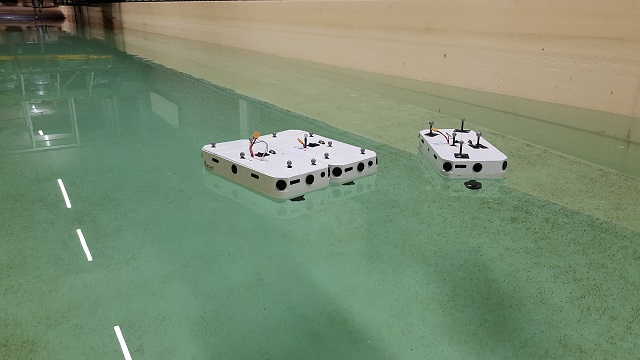
\includegraphics[width=0.6\textwidth]{20210804_171747}
	\caption{Three Delfia-1* modules from RAS Delft in the MTT towing tank facility at 3ME }
	\label{fig:introDelfias}
\end{figure}

\section{Thesis outline}
%This document starts with desribing considerations related to formulating a high level vessel network, it's components. subsystems, agents, and structure. This is followed by a section that focusses on the design choices made on developing the earlier described agents and subsystems. Control strategies in those subsystems will be discussed together with the algorythms that are developed to realize the system behavior. 
The content of this report is as follows:
Chapter 2 answers subquestion 1 by means of literature research on vessel platforming systems and related topics. 
Chapter 3 shows system analysis of behavior A \& B independently, to then predict how functions, requirements, constraints and other characteristics translate and interact in a single system that shows both behaviors which answers subquestion 2.
Chapter 4 describes the proposed multi-vessel and platform state description and a novel approach to predicting dynamics of combined waterborne structures from module models.
Chapter 5 shows the process of designing an implementation of such a system for model scale vessels, to answer subquestion 4. Design choices and considerations are discussed from a high level (a nework) to a low level (behavior of agents within the network) view. 
Chapter 6 aims to analyse performance of the developed framework, by evaluating behavioural responses, thus answering subquestion 5.
Chapter 7 concludes and discusses the findings of this thesis, and finalizes with future recommendations and vision.

Furthermore appendices include (\ref{appendix:techreport})a technical paper that summarizes the work in this project, (\ref{appendix:CombineDynamics}) derivation of the approach to approximate platform dynamics and \ref{appendix:algorythsms} sourcecode of the main algorythms that make up the implemented control software. 